%!TEX root = volumeFinal.tex 

\chapter{\label{chap:results}Resultados - Avaliação de Desempenho}

Foram utilizados três mapas para avaliar o desempenho do algoritmo.
A avaliação dos resultados está divida por mapa.
Em cada mapa é possível jogar em dois lados.
O lado azul começa o jogo na parte superior do mapa, e o lado vermelho começa na parte inferior.
Em cada mapa é avaliado a porcentagem de vitórias para cada domínio.
Os adversários, utilizados para testar o algoritmo, são as técnicas presentes no MicroRTS apresentadas na Seção~\ref{sec:tecn}.
Cada adversário foi utilizado dez vezes em cada mapa, e em cada lado do jogo.

\section{Mapa 1}

No primeiro mapa, cada jogador inicia com uma base, um \textit{worker} e dois recursos próximos a sua base.
O mapa é formado por 16x16 posições.
O lado azul e o lado vermelho tem a mesma formação dos componentes iniciais.
A Figura~\ref{fig:mapa16x16} ilustra a tela do jogo com a configuração inicial do mapa.

\begin{figure}[ht]
	\centering
	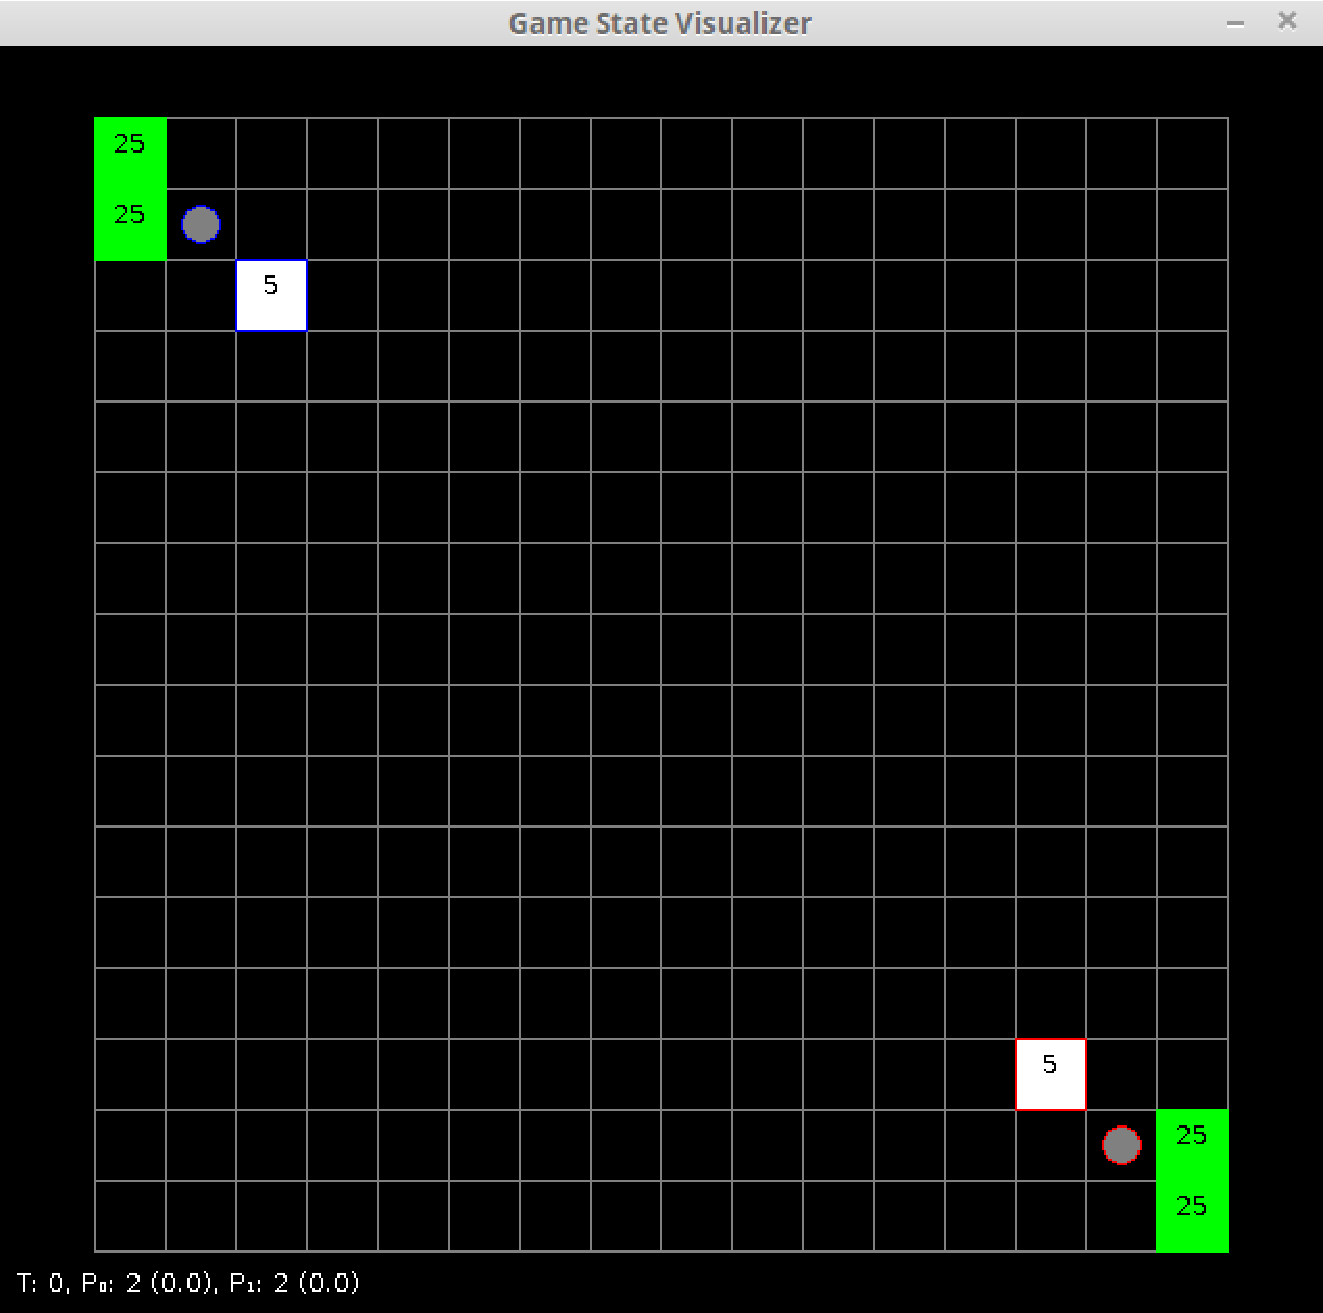
\includegraphics[width=.5\textwidth]{fig/map16x16.pdf}
	\caption{Configuração inicial do mapa 1.}
	\label{fig:mapa16x16}
\end{figure}


A Tabela~\ref{tab:mapa1} ilustra os resultados obtidos com o algoritmo de AHTN contra as técnicas do MicroRTS.
Quando o domínio 1 é executado do lado vermelho, ocorre a criação de duas unidades de ataque ao invés de uma.
Isso ocorre porque o tempo de criação da unidade é maior que o da geração de outra ação do algoritmo.
Quando o algoritmo é invocado novamente, ele não tem conhecimento da unidade que está prestes a ser criada, e assim ocorre a duplicação dessa outra unidade.
O tempo de espera para que o algoritmo gere outra ação foi alterado para tentar remover esse problema.
Mas com um tempo maior, as outras ações eram afetadas, e o algoritmo se torna menos vitorioso.

\begin{table}[ht]
	\centering
	\caption{Porcentagem de vitórias do AHTN no mapa 1.}
	\label{tab:mapa1}
	\begin{tabular}{|c|cc|cc|}
		\hline
		\textbf{}           & \multicolumn{2}{c|}{\textbf{Domínio 1}}  & \multicolumn{2}{c|}{\textbf{Domínio 2}}  \\ \hline
		\textbf{Adversário} & \textbf{Lado Azul} & \textbf{Lado Vermelho} & \textbf{Lado Azul} & \textbf{Lado Vermelho} \\ \hline
		RandomIA            & 100\%              & 100\%                  & 100\%              & 100\%                  \\ \hline
		RandomBiasedIA      & 80\%               & 100\%                  & 100\%              & 100\%                  \\ \hline
		RangedRush          & 0\%                & 100\%                  & 100\%              & 100\%                  \\ \hline
		HeavyRush           & 0\%                & 100\%                  & 0\%                & 100\%                  \\ \hline
		LightRush           & 0\%                & 100\%                  & 0\%                & 100\%                  \\ \hline
		WorkerRush          & 0\%                & 0\%                    & 0\%                & 0\%                    \\ \hline
		MonteCarlo          & 60\%               & 80\%                   & 100\%              & 100\%                  \\ \hline
		Minimax             & 100\%              & 100\%                  & 100\%              & 100\%                  \\ \hline
		Portfolio           & 0\%                & 0\%                    & 0\%                & 0\%                    \\ \hline
	\end{tabular}
\end{table}

A partir dos dados da tabela é possível observar que há um ganho do lado vermelho em relação ao azul nos dois domínios. 
A ação de construir o quartel, gerada pela camada de abstração do MicroRTS, encontra uma posição mais favorável do lado vermelho.
Fazendo com que o lado vermelho tenha uma melhor fluidez na hora da criação das tropas.
O domínio 2 consegue melhores resultados do que o domínio 1.
Adversários que não são vencidos no lado azul passam a ser vencidos com o segundo domínio, e os resultados do lado vermelho são consolidados.

\section{Mapa 2}

Neste mapa, cada jogador inicia com uma base, um \textit{worker}, um quartel e um recurso perto de sua base.
O mapa é composto por 8x8 posições.
O quartel está construído no limite superior do mapa para o jogador azul, e no limite inferior do mapa para o jogador vermelho.
A Figura~\ref{fig:mapa8x8quartel} ilustra a tela do jogo com a configuração inicial do mapa.

\begin{figure}[ht]
	\centering
	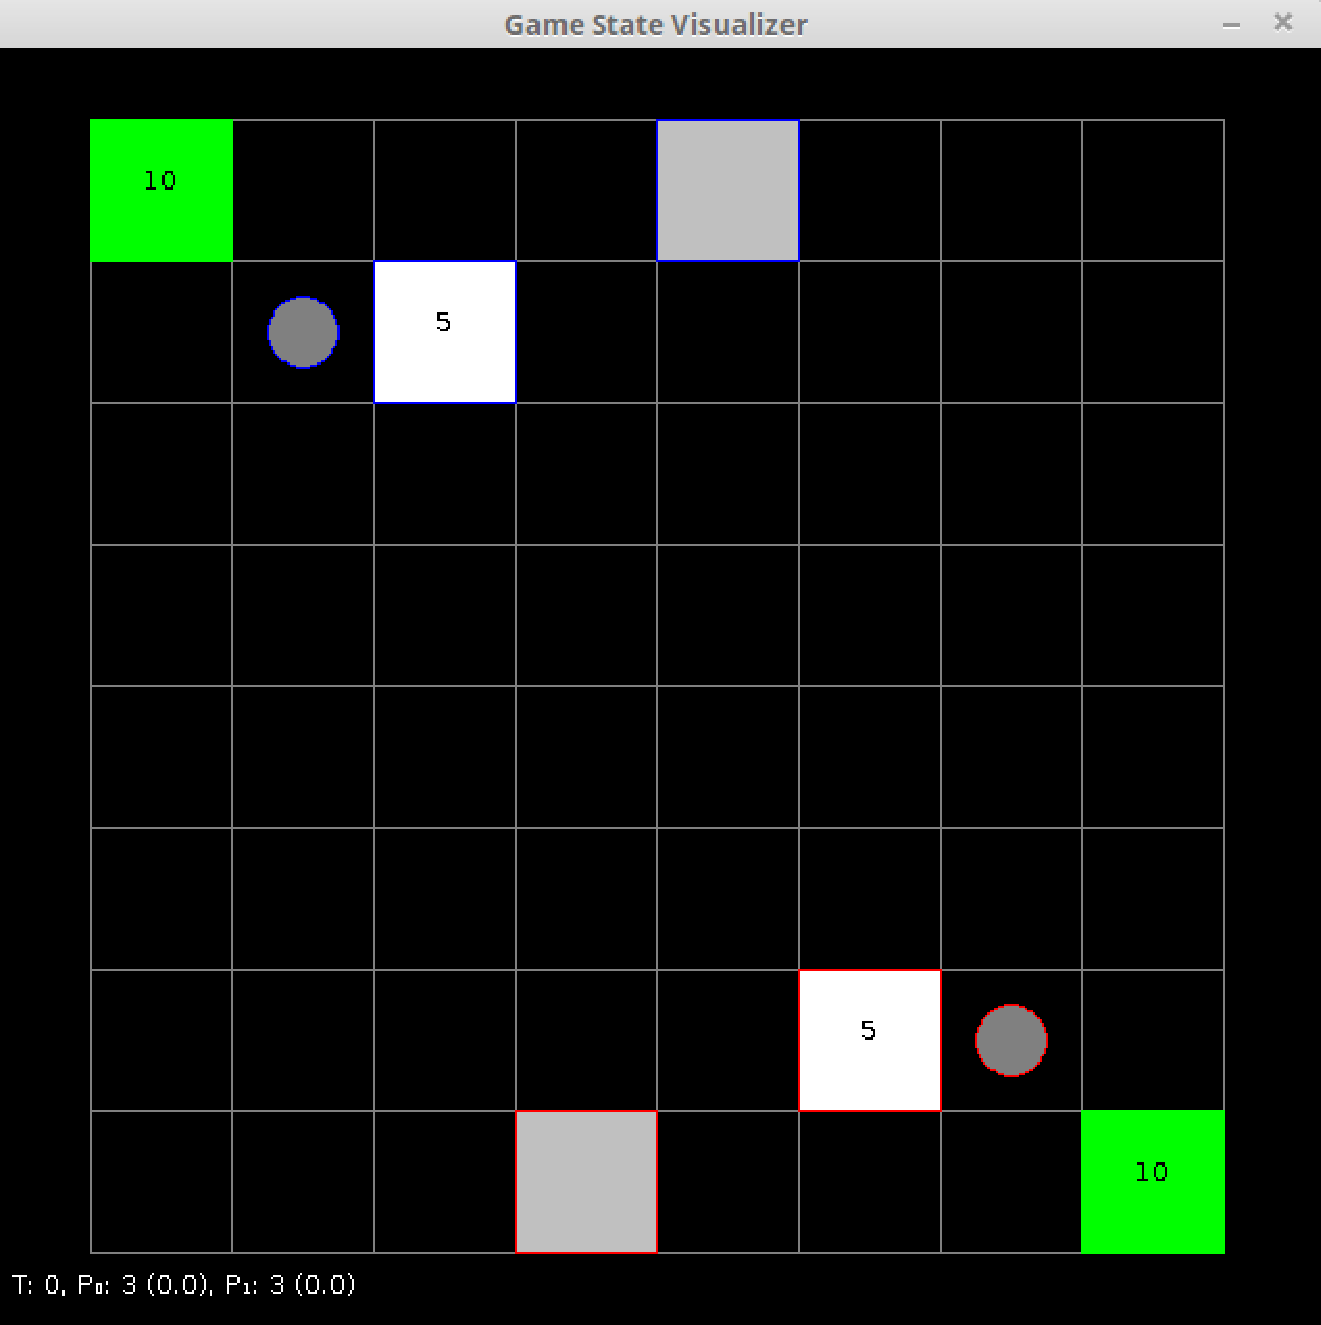
\includegraphics[width=.5\textwidth]{fig/map8x8quartel.pdf}
	\caption{Configuração inicial do mapa 2.}
	\label{fig:mapa8x8quartel}
\end{figure}

A Tabela~\ref{tab:mapa2} ilustra os resultados obtidos neste mapa.
Por conta do mapa ser pequeno em relação ao anterior, não há grande diferença entre os domínios.
O jogo acaba rápido, pois as técnicas criam unidades e logo encontram as unidades adversárias.
Mais uma vez o lado vermelho tem larga vantagem sobre o lado azul. 
Isso acontece pelo fato de que, no lado vermelho, as técnicas do MicroRTS atacam rapidamente, o que não acontece quando as técnicas estão do lado azul, pois após as unidades serem criadas, elas ficam muito tempo paradas antes de atacar.
A técnica do Minimax por exemplo, no lado azul ela cria unidades de ataque mas não envia para atacar, no lado vermelho as tropas são imediatamente postas ao ataque.

\begin{table}[ht]
	\centering
	\caption{Porcentagem de vitórias no mapa 2.}
	\label{tab:mapa2}
	\begin{tabular}{|c|cc|cc|}
		\hline
		\textbf{}           & \multicolumn{2}{c|}{\textbf{Domínio 1}}  & \multicolumn{2}{c|}{\textbf{Domínio 2}}  \\ \hline
		\textbf{Adversário} & \textbf{Lado Azul} & \textbf{Lado Vermelho} & \textbf{Lado Azul} & \textbf{Lado Vermelho} \\ \hline
		RandomIA            & 100\%              & 100\%                  & 100\%              & 100\%                  \\ \hline
		RandomBiasedIA      & 40\%               & 80\%                   & 80\%               & 100\%                  \\ \hline
		RangedRush          & 0\%                & 100\%                  & 0\%                & 100\%                  \\ \hline
		HeavyRush           & 0\%                & 100\%                  & 0\%                & 100\%                  \\ \hline
		LightRush           & 0\%                & 100\%                  & 0\%                & 100\%                  \\ \hline
		WorkerRush          & 0\%                & 0\%                    & 0\%                & 0\%                    \\ \hline
		MonteCarlo          & 0\%                & 0\%                    & 0\%                & 0\%                    \\ \hline
		Minimax             & 0\%                & 100\%                  & 0\%                & 100\%                  \\ \hline
		Portfolio           & 0\%                & 60\%                  & 0\%                & 80\%                  \\ \hline
	\end{tabular}
\end{table}

\section{Mapa 3}

Neste mapa, cada jogador inicia com uma base, um \textit{worker}, e um recurso perto de sua base.
O mapa é composto por 8x8 posições.
Além dos componentes dos jogadores, há posições obstáculos no centro do mapa.
Os obstáculos não são posições validas para os jogadores.
A Figura~\ref{fig:mapa8x8obsta} ilustra a tela do jogo com a configuração inicial do mapa.

\begin{figure}[ht]
	\centering
	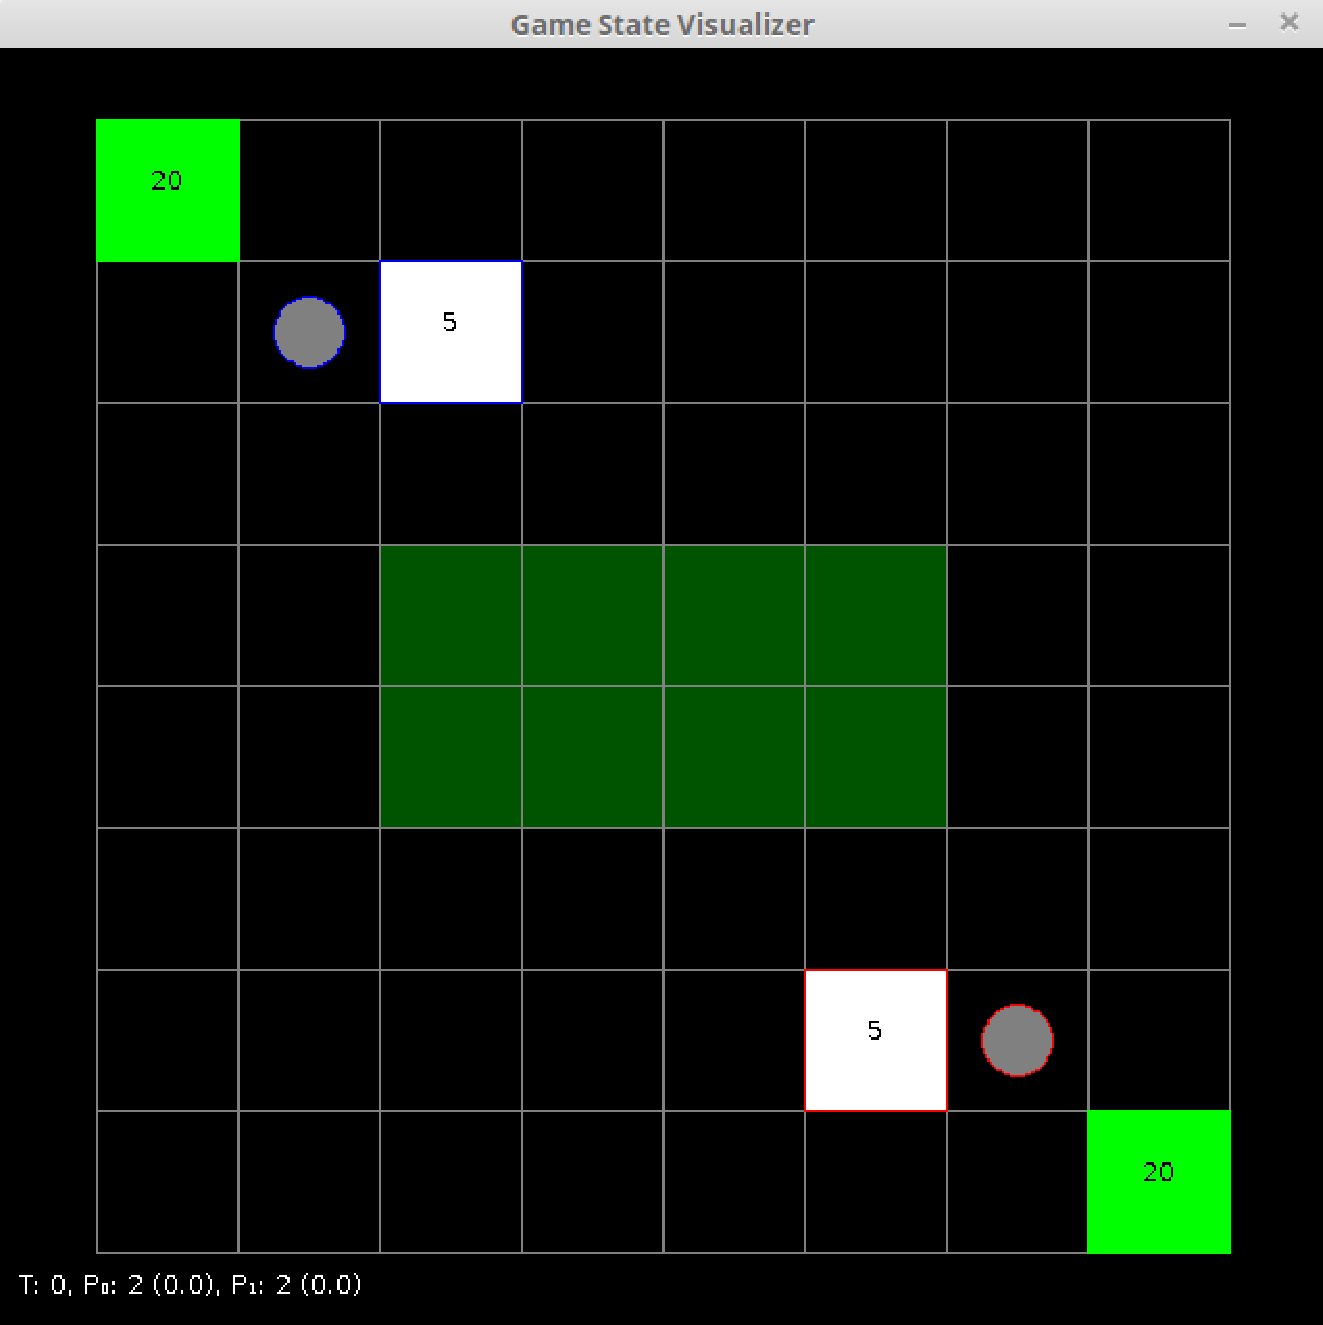
\includegraphics[width=.5\textwidth]{fig/map8x8obsta.pdf}
	\caption{Configuração inicial do mapa 3.}
	\label{fig:mapa8x8obsta}
\end{figure}

A Tabela~\ref{tab:mapa3} ilustra os resultados obtidos neste mapa.
Os resultados mostram, outra vez, a vantagem do lado vermelho no jogo.
Do mesmo modo que no mapa 1, a construção do quartel é mais favorável do lado vermelho.
A colocação de obstáculos no mapa não alterou a maneira com que as técnicas se comportam.

\begin{table}[ht]
	\centering
	\caption{Porcentagem de vitórias no mapa 3.}
	\label{tab:mapa3}
	\begin{tabular}{|c|cc|cc|}
		\hline
		\textbf{}           & \multicolumn{2}{c|}{\textbf{Domínio 1}}  & \multicolumn{2}{c|}{\textbf{Domínio 2}}  \\ \hline
		\textbf{Adversário} & \textbf{Lado Azul} & \textbf{Lado Vermelho} & \textbf{Lado Azul} & \textbf{Lado Vermelho} \\ \hline
		RandomIA            & 100\%              & 100\%                  & 100\%              & 100\%                  \\ \hline
		RandomBiasedIA      & 100\%              & 80\%                   & 100\%              & 80\%                   \\ \hline
		RangedRush          & 0\%                & 100\%                  & 0\%                & 100\%                  \\ \hline
		HeavyRush           & 0\%                & 100\%                  & 0\%                & 100\%                  \\ \hline
		LightRush           & 0\%                & 100\%                  & 0\%                & 100\%                  \\ \hline
		WorkerRush          & 0\%                & 0\%                    & 0\%                & 0\%                    \\ \hline
		MonteCarlo          & 0\%                & 0\%                    & 0\%                & 0\%                    \\ \hline
		Minimax             & 0\%                & 80\%                  & 80\%              & 80\%                   \\ \hline
		Portfolio           & 0\%                & 0\%                    & 0\%                & 0\%                    \\ \hline
	\end{tabular}
\end{table}

A técnica de WorkerRush não é vencida em nenhuma configuração de jogo.
Isso acontece porque, a técnica treina \textit{workers}, que é a unidade que custa menos no jogo, e logo as envia para atacar, por essa razão o algoritmo não tem tempo de ter algum tipo de reação.
A técnica de Portfolio perde apenas no mapa 2, pois as tropas ficam um tempo parada antes de atacar, o que não acontece nos outros mapas.
O tempo parado faz com que o algoritmo de AHTN consiga gerar as ações necessárias para que unidades de ataque sejam criadas.

O grande problema dos domínios modelados é não ter um plano de contingencia.
O adversário pode estar criando muitas tropas, mas o domínio segue o plano de criar suas unidades de ataque, o que leva o adversário a vitoria.
Os domínios perdem contra técnicas que treinam unidades de ataque de forma rápida, por causa do tempo que leva para construir um quartel e revidar ao ataque.

 

\section{Tamanho de cada IA}

Algumas técnicas podem precisar de muito esforço de programação para serem implementadas, já outras podem ser feitas de maneira mais rápida e ter a mesma eficiência.
Uma maneira de comparar as técnicas é através do tamanho do código.
Assim é possível ver o esforço empregado na criação das técnicas.
Pois quanto maior o tamanho, maior o número de linhas de código necessários para a implementação da técnica.
A Tabela~\ref{tab:tamanho} ilustra o tamanho de cada técnica após aplicado um algoritmo de compressão de dados.

\begin{table}[ht]
	\centering
	\caption{Tamanho do código de cada técnica.}
	\label{tab:tamanho}
	\begin{tabular}{|c|c|}
		\hline
		\textbf{Adversário}     & \textbf{Tamanho} \\ \hline
		Domínio HTN 1           & 19,9 kB          \\ \hline
		Domínio HTN 2           & 20,1 kB          \\ \hline
		RandomIA                & 4,0 kB           \\ \hline
		RandomBiasedIA          & 4,6 kB           \\ \hline
		RangedRush              & 13,7 kB          \\ \hline
		HeavyRush               & 14,0 kB          \\ \hline
		LightRush               & 14,0 kB          \\ \hline
		WorkerRush              & 13,6 kB          \\ \hline
		MonteCarlo              & 18,1 kB          \\ \hline
		Minimax                 & 12,9 kB          \\ \hline
		Portfolio               & 14,4 kB          \\ \hline
	\end{tabular}
\end{table}

A implementação do algoritmo de AHTN é a técnica com maior tamanho.
Isso vem do fato de que é preciso integrar com o algoritmo as classes do JSHOP2 e a camada de abstração do MicroRTS.
Fazendo com que o tamanho do código cresça.

A técnica com maior tamanho do MicroRTS é a MonteCarlo.
Contra o algoritmo de AHTN, essa técnica venceu sempre nos mapas 2 e 3, e perdeu no mapa 1 para o domínio 2.
A técnica WorkerRush é a única que não perde em nenhum cenário de jogo.
Ela possui tamanho perto da media dos tamanhos.
As técnicas mais simples, que apenas utilizam movimentos aleatórios, são as técnicas de menor tamanho, e ainda em alguns casos conseguem vencer.

\section{Tempo de geração das ações}

Em jogos RTS, o tempo de geração de uma ação é fundamental.
Técnicas que demoram muito tempo para gerar as ações tendem a ser superadas.
Isso ocorre porque o jogador adversário tem mais tempo para executar suas ações.

A técnica de LightRush foi escolhida como adversário para avaliar o tempo de geração das ações no algoritmo de AHTN.
Essa técnica foi escolhida por ter o mesmo comportamento contra os dois domínios.
O mapa 1 foi o mapa utilizado para este teste.
A Figura~\ref{fig:tempo} ilustra o gráfico com os tempos obtidos para os domínios.

\begin{figure}[ht]
	\centering
	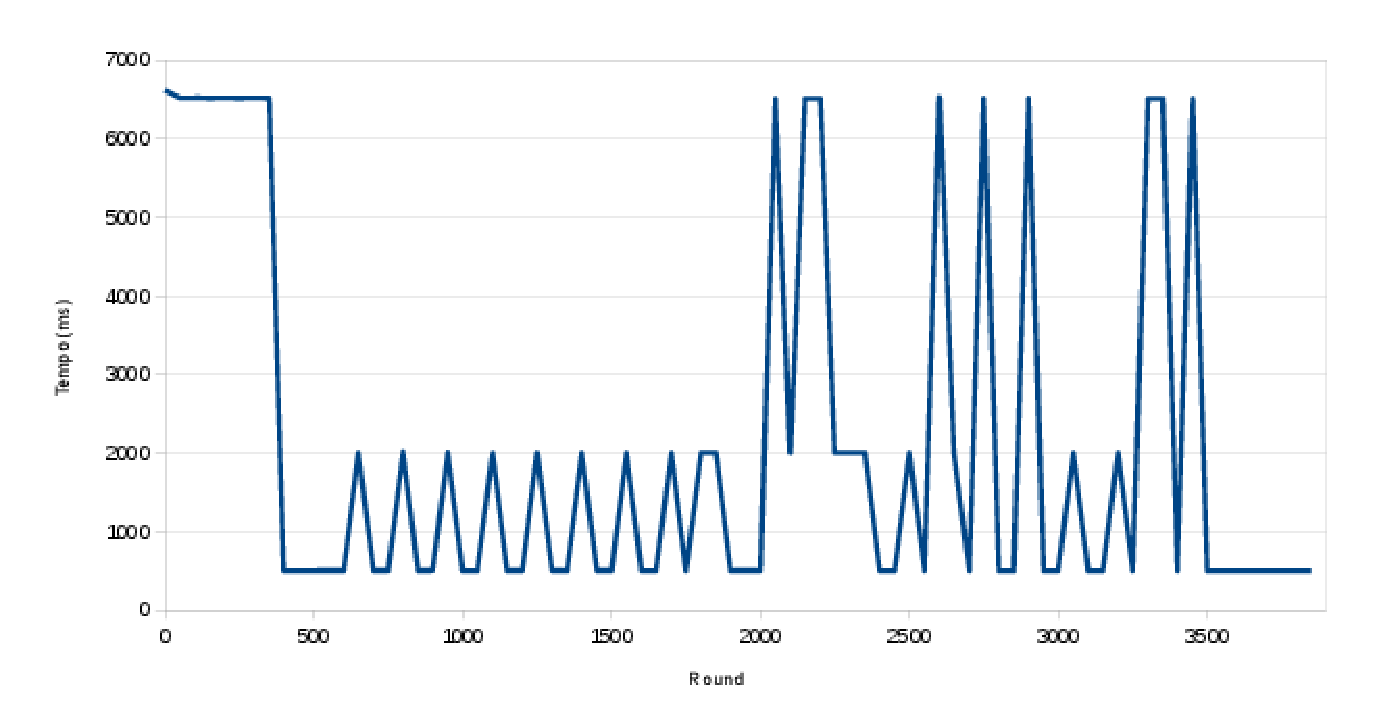
\includegraphics[width=.9\textwidth]{fig/graph.pdf}
	\caption{Tempo de geração das ações para os dois domínios.}
	\label{fig:tempo}
\end{figure}

O gráfico mostra que no inicio do jogo o tempo para gerar uma ação é elevado.
No inicio do jogo, o jogador tem apenas uma base e um \textit{worker}.
Para conseguir vencer o adversário é preciso construir um quartel, e treinar unidades de ataque.
Ao passar das jogadas, o tempo para gerar as jogadas diminui.
Isso ocorre porque há menos ações que podem ser realizadas no jogo, o que implica em menos níveis na árvore de busca que o algoritmo tem que percorrer.
No final do jogo, o jogador já tem tropas de ataque e apenas manda elas atacar.

No domínio 1 o tempo de gerar a unidade de ataque é menor do que no domínio 2.
Isso acontece, pelo fato de que no domínio 1, apenas uma unidade é criada, e com isso os planos gerados são diferentes, já no domínio 2 mais de uma unidade é criada.
O tempo de geração ao final do jogo é semelhante, pois as duas abordagens são parecidas, e se diferem apenas na maneira como as unidades são criadas.

As técnicas do MicroRTS conseguem gerar as ações em poucos milissegundos.
Já o algoritmo de AHTN implementado leva no minimo meio segundo para determinar qual ação deve ser realizada.
Isso ocorre por causa de que a cada troca de perspectiva, o algoritmo tem que gerar os planos novamente.
Pois a cada novo nível na árvore de busca algum componente do ambiente mudou.


